\section{Implement and Test}

\subsection{Description}

\noindent\fbox{
	\parbox{\textwidth}{
		\textbf{5.} Select the SysML/UML model for your preferred architecture suggestions in \textbf{3.} Choose a part of the functionality including both hardware and software components to create a model and a testbench in HLS using SystemC or C-code. Simulate and validate your design model. \\\\
		Argue for your choice of modeling language and abstraction level of modeling. Use the reports from the HLS tool to evaluate performance of the design. Assess whether the design is able to fulfill your requirements and constraints.
	}
}\citepawesome{Bjerge2017}{2}
\\\\

\subsection{Float as a Datatype}
Throughout this project, it has not been stated how essential it is that the data worked on is as close to real values as possible. Using long double as the used datatype both for calculation and evaluation for the particle swarm optimization algorithm is preferred. This is the floating point with most precision supported in SystemC. Working with Vivado  however, it is known that only fix point as a datatype is supported. To keep it simple the students have created a test program in the Vivado HLS tool that uses floats as a datatype both for calculations and in data transfers, to check if it is possible to use floating point, without conversion, when trying to hardware accelerate. The program that will be introduced in this section is floatPrototype.\\

The minimal design of floatPrototype is a IP core that take in two inputs, of type float, make a simple calculation with the data and returns it as a float. This will show that all the basic building blocks of the desired functionality in the PSOS can be achieved. On Figure \ref{fig:floatprototype} is a basic drawing of the desired flow of the floatPrototype IP core.\\

\begin{figure}[H]
	\centering
	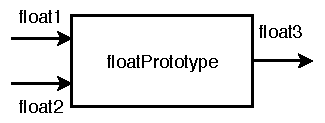
\includegraphics[width=0.5\linewidth]{diagram/floatPrototype}
	\caption{Figure showing the flow of floatPrototype.}
	\label{fig:floatprototype}
\end{figure}




\begin{lstlisting}[style=customc++, label={lst:floatPrototype.h}, caption={Simplified view of the header file of floatPrototype.}]
[...]
SC_MODULE(floatPrototypec){
[...]
  sc_in<float> float1;
  sc_in<float> float2;
  sc_out<float> float3;
  
  void multiply();
[...]
\end{lstlisting}

On Listing \ref{lst:floatPrototype.h} and \ref{lst:floatPrototype.cpp} is the SystemC implementation of floatPrototype, scaled down to the core of the IP core test. As can be seen on Listing \ref{lst:floatPrototype.h} the IP core that is being created has two float inputs, \texttt{float1} and \texttt{float2}, as well as a float output, \texttt{float3}. It has a function, \texttt{multiply()}, which simply multiplies \texttt{float1} with \texttt{float2} and writes the result onto \texttt{float3}.

\begin{lstlisting}[style=customc++, label={lst:floatPrototype.cpp}, caption={SystemC file of floatPrototype.}]
#include "floatPrototype.h"

void floatPrototypec::multiply(){
  #pragma HLS resource core=AXI4LiteS metadata="-bus_bundle slv0" variable=float1
[...]
  float3.write( float1.read() * float2.read() );
}
\end{lstlisting}

A simulation of the code is constructed and conducted in the Vivado HLS tools. The specific test is not included in this section. If study of the test is desired, the reader is referred to the HLS appendix that can be found in the "appendix.zip". The outcome of the test suit is the expected outcome in the case that the program functions using floats. The summary after the synthesis of floatPrototype can be seen on Figure \ref{fig:floatprototypesynthesissummary}.\\

\begin{figure}[H]
	\centering
	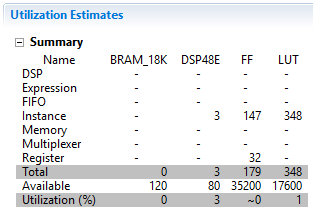
\includegraphics[width=0.5\linewidth]{diagram/floatPrototype_synthesis_summary}
	\caption{Autogenerated summary after synthesis of floatPrototype}
	\label{fig:floatprototypesynthesissummary}
\end{figure}


To further elaborate upon the float as a datatype test, the floatPrototype is exported as an RTL from the Vivado HLS tool, and included into a simple program in which tests are conducted to check whether it is possible to utilize floats in an IP core with the datatype being transferred directly.

%TODO indsæt Vivado test af floatPrototype her!!!

\subsection{Vivado}%TODO find ud af om det er den rigtige chip der er stated
This section show the implementation of different software patterns onto the Zynq chip. The design makes use of the GPIO ports to access the hardware buttons and switches, to control the state of the PSOS, as shown on Figure \ref{fig:smdguistate}, on page \pageref{fig:smdguistate}. The buttons are used to control the actions in the application ActionUp, ActionDown, ActionNext and ActionStart. The switches are used to control the different of the PSOS; Setup, FindMinima and FindMaxima.

INSERT IMAGE OF BLOCK DIAGRAM FROM Verdado!!!!!!

The Software is made using FreeRTOS, where the mainThread controls the application. As it can be seen below it initializes the buttons and switches.

\begin{lstlisting}[style=customc++, label={lst:listingExample}, caption={Example listing.}]
#include <stdio.h>
#define N 10
/* Block
* comment */
{

INSERT CODEEEEEEEEEEEEEEEEEEEEEEEEEEEEEEEEEEEEEEEEEEEEEEEE

}
\end{lstlisting}

As menshioned in section \ref{designpatterns} the gof state patteren is used. The context can be seen below.
\begin{lstlisting}[style=customc++, label={lst:listingExample}, caption={Example listing.}]
#include <stdio.h>
#define N 10
/* Block
* comment */
{

INSERT CODEEEEEEEEEEEEEEEEEEEEEEEEEEEEEEEEEEEEEEEEEEEEEEEE

}
\end{lstlisting}

The states is an important part of this patterens therefore an example of the setup state can be seen here. To make the code easier to read it is clearly split into actions and transitions. 


\subsection{Vivado HLS}

\subsection{Description}

\noindent\fbox{
	\parbox{\textwidth}{
		\textbf{6.} Implement and test a part of your system using the ZYBO platform including at least one IP core written and verified with the HLS tool.
	}
}\citepawesome{Bjerge2017}{2}